\documentclass{article}

% This draft follows the NeurIPS 2026 file pasted by the student.
% If the course provides neurips_2019.sty instead, replace only the next line
% with \usepackage[preprint]{neurips_2019}; do not edit the style file itself.
\usepackage[preprint]{neurips_2026}
\usepackage[utf8]{inputenc}
\usepackage[T1]{fontenc}
\usepackage{hyperref}
\usepackage{url}
\usepackage{booktabs}
\usepackage{amsmath}
\usepackage{amsfonts}
\usepackage{nicefrac}
\usepackage{microtype}
\usepackage{xcolor}
\usepackage{graphicx}

\newcommand{\tbd}[1]{\textcolor{red}{[TBD: #1]}}

\title{Can Quality-Aware Data Augmentation Improve the Robustness of Pneumonia Classification Under Chest X-Ray Degradation?}

\author{%
  DUAN YUGUANg \\
  G2610013E \\
  MD6329: Deep Learning for Healthcare AI \\
  Lee Kong Chian School of Medicine, Nanyang Technological University \\
  \texttt{YUGUANg003@e.ntu.edu.sg} \\
}

\begin{document}

\maketitle

\begin{abstract}
Deep-learning systems can classify pneumonia from chest radiographs, but their performance may deteriorate when images have blur, noise, low contrast, or reduced effective resolution. We investigate whether quality-aware data augmentation improves this robustness without sacrificing clean-image performance. On the binary PneumoniaMNIST benchmark, we compare a compact residual convolutional neural network (CNN) and a compact Vision Transformer (ViT), each trained either on clean images only or with moderate, label-preserving quality perturbations. The augmentation policy samples Gaussian blur, additive noise, contrast reduction, or downsampling followed by upsampling during training only. We evaluate the four models on a held-out clean test set and on matched, deterministically corrupted versions of the same images. The primary outcome is area under the receiver operating characteristic curve (AUROC); average precision, balanced accuracy, macro-F1, sensitivity, and specificity are secondary outcomes. For the CNN, augmentation improved clean AUROC from 0.955 to 0.962 and mean degraded AUROC from 0.907 to 0.948. For the ViT, clean AUROC changed from 0.953 to 0.951 and mean degraded AUROC remained 0.934. Thus, this policy substantially improved CNN robustness without an observed clean-image penalty, but did not produce an aggregate robustness gain for the ViT in this single-seed experiment.
\end{abstract}

\section{Problem formulation}

\subsection{Clinical motivation}

Chest radiography is frequently used when pneumonia is suspected, and deep-learning systems have shown that chest X-ray images can support automated pneumonia classification \citep{kermany2018,rajpurkar2017}. However, a radiograph seen by a model is not always an idealized image. Acquisition settings, patient motion, detector noise, contrast processing, compression, and limited spatial resolution can alter its appearance. A classifier that performs well only on clean benchmark images may therefore be unreliable when image quality shifts at deployment.

This concern is especially important in medical imaging, where a model can achieve apparently strong internal performance while relying on non-pathological cues. In a multi-hospital pneumonia study, \citet{zech2018} found that generalization varied across hospital systems and that acquisition-related information could be predictive of model outputs. More broadly, \citet{degrave2021} demonstrated shortcut learning in chest-radiograph models. These findings motivate an explicit evaluation of sensitivity to image-quality change rather than reporting clean-test performance alone. The present study is deliberately narrow: it evaluates controlled synthetic degradations in a benchmark dataset; it does not claim to validate a diagnostic system for clinical deployment.

\subsection{Research question and hypotheses}

Our research question is: \emph{Can quality-aware data augmentation improve the robustness of pneumonia classification models to degraded chest X-rays without sacrificing performance on clean images?}

For an architecture $a$, let $\operatorname{AUROC}_{a,c}$ denote its test AUROC under condition $c$ and let $\mathcal{C}_{\mathrm{deg}}$ be the seven degraded conditions. We summarize degraded robustness by
\[
R_a=\frac{1}{|\mathcal{C}_{\mathrm{deg}}|}\sum_{c\in\mathcal{C}_{\mathrm{deg}}}\operatorname{AUROC}_{a,c}.
\]
The augmentation effect is evaluated within an architecture, i.e., $R_{C1}-R_{C0}$ for the CNN and $R_{T1}-R_{T0}$ for the ViT. We test two pre-specified hypotheses:
\begin{itemize}
    \item \textbf{H1 (robustness):} quality-aware augmentation increases mean AUROC across degraded test conditions relative to the same architecture trained on clean images only.
    \item \textbf{H2 (clean-image preservation):} quality-aware augmentation does not materially decrease clean-test AUROC. For this small benchmark study, we define a material decrease operationally as more than 0.02 AUROC; this is a reporting criterion rather than a formal equivalence test.
\end{itemize}

\subsection{Contributions}

This report makes three limited contributions. First, it evaluates controlled quality degradation rather than clean accuracy alone. Second, it estimates the effect of one fixed augmentation policy separately in a CNN and a ViT. Third, it reports clean and corruption-specific metrics, allowing any robustness gain to be interpreted alongside a possible clean-image trade-off. This is a benchmark study, not a clinically validated diagnostic system.

\subsection{Use of Software 3.0 and generative AI}

AI copilots were used to support project brainstorming, code organization, debugging, and the initial drafting of the report structure. The author reviewed the dataset handling, experimental settings, metric calculations, cited sources, and final written claims. Generative AI was not used to generate labels, alter the images, or determine reported numerical results. This disclosure should be revised if it does not accurately describe the author's final workflow.

\section{Related work}

\subsection{Pneumonia classification and benchmark datasets}

Kermany et al. demonstrated deep learning for pediatric pneumonia classification from chest X-rays \citep{kermany2018}, while CheXNet popularized large-scale chest-radiograph classification with a DenseNet-121 model \citep{rajpurkar2017}. These studies establish the clinical relevance of automated chest-radiograph interpretation, but a high internal-test score alone does not establish reliability under distribution shift. PneumoniaMNIST, used here, is a standardized binary chest-X-ray subset within MedMNIST v2 with predefined training, validation, and test splits \citep{yang2023}. Its compact, fixed format makes it suitable for a reproducible comparison, although its scale and pediatric source limit its clinical scope.

\subsection{Generalization and shortcut learning}

Generalization is a central concern for medical-image models. \citet{zech2018} reported lower performance when pneumonia models were evaluated on radiographs from external hospital systems and showed that hospital-system information could be strongly encoded in images. \citet{degrave2021} likewise demonstrated that chest-radiograph classifiers can exploit confounding features rather than pathology. Quality degradation is not identical to hospital shift, but it is one concrete source of appearance change that can be isolated experimentally. Accordingly, this study does not claim external validation; it evaluates fixed, reproducible quality corruptions on the same held-out images.

\subsection{Data augmentation and corruption robustness}

Data augmentation is widely used to reduce overfitting and improve generalization when training data are limited \citep{shorten2019}. In chest radiography, \citet{ganesan2019} compared traditional and GAN-based augmentation and found that no augmentation family is uniformly superior. More recent work has examined augmentation choices for chest X-rays and their relationship to robust representations \citep{vandersluijs2024}. Complementarily, common-corruption benchmarks in natural-image vision formalized evaluation under realistic image degradations rather than adversarial perturbations alone \citep{hendrycks2019}. Building on these ideas, we use a deliberately narrow policy: blur, noise, contrast reduction, and reduced resolution represent image-quality changes, whereas large rotations, aggressive crops, and colour transforms might modify anatomy or introduce implausible radiographs.

\subsection{CNNs and Vision Transformers}

Residual CNNs use skip connections to ease optimization of deep image models \citep{he2016}; their locality and translation-oriented inductive bias can be beneficial when data are limited. Vision Transformers represent images as patch tokens and use self-attention to aggregate information globally \citep{dosovitskiy2021}. Comparing these architectures is useful because quality degradations may affect local texture and global structure differently. The comparison is empirical: the study does not assume that either architecture is inherently more robust.

\subsection{Connection to course lecture}

This project connects most directly to the course lecture on \tbd{insert lecture number and title}, especially slides \tbd{insert slide range} and timestamp \tbd{insert video timestamp}. Its discussion of \tbd{insert the relevant concept, e.g., distribution shift, robustness, or data-centric evaluation} motivates evaluating behaviour under a quality shift rather than relying only on in-distribution accuracy. The precise lecture reference must be checked against the course recording before submission.

\section{Data}

\subsection{Dataset and labels}

We use the 128$\times$128 grayscale version of PneumoniaMNIST, a binary pediatric chest-X-ray dataset distributed through MedMNIST v2 \citep{yang2023}. Label 0 denotes \emph{normal} and label 1 denotes \emph{pneumonia}. The released data contain 5,856 images across predefined splits (Table~\ref{tab:data}). The training and validation splits are class imbalanced, with pneumonia images comprising approximately 74\% of each split; the test split has 62.5\% pneumonia images.

\begin{table}[t]
\caption{PneumoniaMNIST split sizes and class counts in the supplied 128$\times$128 NPZ file.}
\label{tab:data}
\centering
\begin{tabular}{lrrr}
\toprule
Split & Normal & Pneumonia & Total \\
\midrule
Training & 1,214 & 3,494 & 4,708 \\
Validation & 135 & 389 & 524 \\
Test & 234 & 390 & 624 \\
\bottomrule
\end{tabular}
\end{table}

The 64, 128, and 224 versions are different-resolution representations of the same dataset rather than independent observations. We use only the 128$\times$128 version in the reported experiments. An exact pixel-hash audit found eight validation images that were duplicates of training images. These validation duplicates were removed before model selection, leaving an effective validation set of 516 images; no conflicting duplicate labels were found. This precaution prevents validation performance from benefiting from exact training-image repetition.

\subsection{Exploratory data analysis}

The EDA included class-distribution summaries, a visual audit of representative normal and pneumonia images, and per-image summaries of mean intensity, contrast, and sharpness. Table~\ref{tab:qualityproxies} reports the median value of each proxy in the training split. Pneumonia images had higher mean intensity but lower contrast and sharpness under these summaries. These are descriptive observations, not evidence that pneumonia images were acquired at lower quality: disease appearance itself may alter intensity and texture. The EDA therefore motivates controlled quality perturbations but is not used as a proxy label for image quality.

\begin{table}[t]
\caption{Training-set median image-quality proxies by class. Values are descriptive and should not be interpreted as causal acquisition-quality differences.}
\label{tab:qualityproxies}
\centering
\begin{tabular}{lrrr}
\toprule
Label & Mean intensity & Contrast & Sharpness \\
\midrule
Normal & 140.44 & 46.49 & 6.47 \\
Pneumonia & 149.92 & 35.97 & 3.77 \\
\bottomrule
\end{tabular}
\end{table}

\subsection{Preprocessing}

Each image is converted from unsigned 8-bit intensity values to the interval $[0,1]$. The global mean and standard deviation are calculated from training images only and used to normalize the training, validation, and test splits. Quality augmentation, when enabled, is applied to a training image before normalization. The predefined test split is not used for early stopping or checkpoint selection. Figure~\ref{fig:dataexamples} should show representative images from both classes; it is retained as a required qualitative data check.

\begin{figure}[t]
\centering
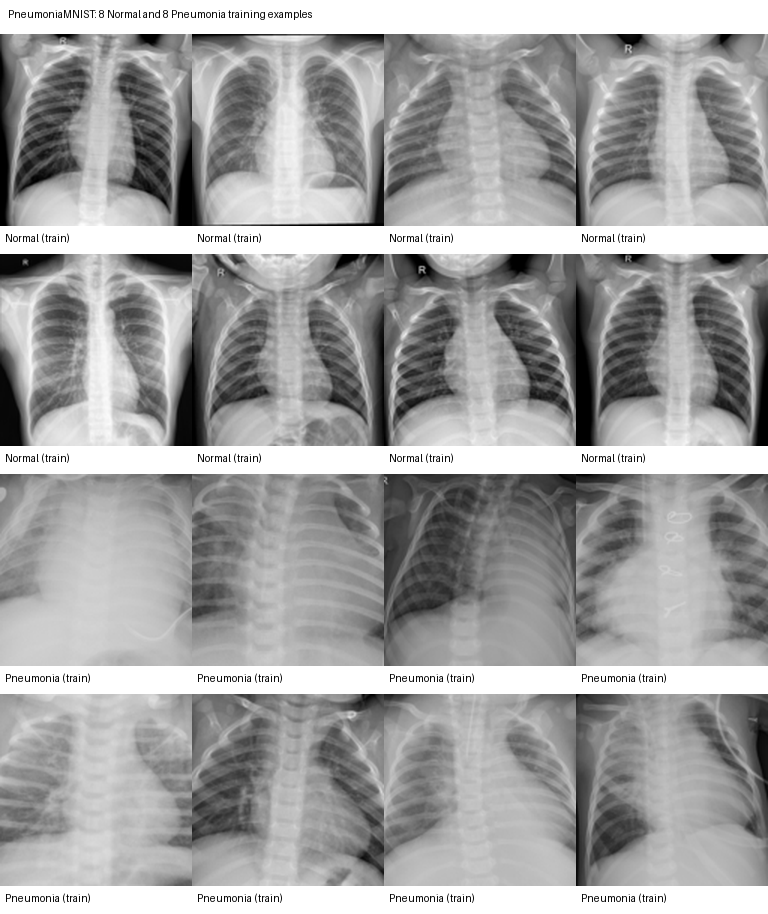
\includegraphics[width=0.96\linewidth]{figures/pneumoniamnist_examples.png}
\caption{Representative PneumoniaMNIST training radiographs. Eight normal examples and eight pneumonia examples were selected with fixed seed 17 for qualitative inspection.}
\label{fig:dataexamples}
\end{figure}

\section{Approach}

\subsection{Experimental design}

We use a $2\times2$ factorial design: architecture (CNN versus ViT) and training policy (clean-only versus quality-aware augmentation). This produces the four runs in Table~\ref{tab:design}. C0 and T0 are the within-architecture controls; C1 and T1 are their corresponding augmentation treatments. All runs use the same dataset split, random seed, evaluation corruptions, and model-selection rule. The primary contrasts are therefore C1--C0 and T1--T0, not an unrestricted claim that one architecture universally outperforms the other.

\begin{table}[t]
\caption{Planned experiments. Augmentation is used only while fitting the training split.}
\label{tab:design}
\centering
\begin{tabular}{llll}
\toprule
ID & Architecture & Training inputs & Purpose \\
\midrule
C0 & CNN & Clean only & CNN baseline \\
C1 & CNN & Clean + quality augmentation & CNN augmentation effect \\
T0 & ViT & Clean only & ViT baseline \\
T1 & ViT & Clean + quality augmentation & ViT augmentation effect \\
\bottomrule
\end{tabular}
\end{table}

\subsection{CNN}

The CNN is a compact ResNet-18-style classifier for single-channel 128$\times$128 images. Its stem uses a 7$\times$7 convolution with 32 channels, batch normalization, ReLU activation, and max pooling. It then uses four residual stages with channel widths 32, 64, 128, and 256; the latter three stages downsample spatially. Each residual block adds its transformed input to an identity or projection shortcut before the final nonlinearity. Global average pooling produces a 256-dimensional feature vector, and a linear layer maps it to two logits. This architecture retains the residual-learning principle of \citet{he2016} while remaining modest relative to the dataset size.

\subsection{Vision Transformer}

The ViT converts the single-channel image into non-overlapping 16$\times$16 patches using a stride-16 convolutional patch embedding. The 128$\times$128 input yields 64 patch tokens. These are combined with a learned class token and learned positional embeddings. The encoder contains six Transformer layers with embedding dimension 256, eight attention heads, a 512-dimensional feed-forward layer, GELU activation, dropout 0.10, residual connections, and layer normalization. The normalized class-token representation is passed to a linear two-logit classification head. The model is trained from scratch rather than initialized from a natural-image pretrained ViT, keeping the architecture comparison focused on the stated training data and augmentation policy.

\subsection{Quality-aware augmentation}

For C1 and T1, one moderate quality perturbation is sampled with probability 0.75 for each training image; otherwise the image remains clean. Conditional on augmentation, the perturbation type is chosen uniformly from: (i) Gaussian blur with $\sigma\in[0.35,1.25]$ pixels; (ii) additive Gaussian noise with standard deviation in $[0.01,0.05]$ on the $[0,1]$ intensity scale; (iii) contrast scaling around the image mean by a factor in $[0.60,1.00]$; and (iv) downsampling to 50--85\% of the original linear size followed by bilinear upsampling. Pixel intensities are clipped to $[0,1]$ after applicable transforms. The diagnostic label is unchanged because the perturbations simulate moderate acquisition-quality variation rather than a biological change. No horizontal flipping, large rotation, aggressive cropping, or colour augmentation is used, because the purpose is to model image quality rather than create anatomically implausible chest radiographs. C0 and T0 receive only the common preprocessing described in Section~3.2.

\subsection{Training}

Both models are trained with class-weighted cross-entropy. For class $c$, the weight is $w_c=N/(2n_c)$, where $N$ is the number of training images and $n_c$ is the number belonging to class $c$. For a sample with one-hot label $y$ and predicted class probabilities $p$, the loss is $\mathcal{L}=-\sum_c w_c y_c\log p_c$. This weighting counters the approximately 3:1 pneumonia-to-normal class imbalance in the training split.

Optimization uses AdamW with weight decay $10^{-4}$, batch size 32, a cosine-annealing learning-rate schedule, and a maximum of 35 epochs. The CNN uses an initial learning rate of $3\times10^{-4}$ and the ViT uses $1\times10^{-4}$. Training stops after eight consecutive epochs without improvement in validation AUROC, and the checkpoint with the highest validation AUROC is retained. The seed is 17. \tbd{Before submission, add the exact device, PyTorch version, and wall-clock duration of each final run from the experiment log.}

\section{Experiments}

\subsection{Evaluation protocol and metrics}

Each selected checkpoint is evaluated first on the clean test set, then on exactly the same test images under fixed degradations: Gaussian blur ($\sigma=1.0$ and $2.0$), Gaussian noise (standard deviation 0.03 and 0.07), contrast factors 0.60 and 0.35, and downsample--upsample at scale 0.50. Test corruption is deterministic for a given image index and seed. Augmentation is never applied to validation images or clean test images. The checkpoints selected by validation AUROC were from epochs 13 (C0), 4 (C1), 10 (T0), and 17 (T1); eight validation duplicates were removed consistently in every run.

The primary metric is AUROC, which summarizes discrimination across thresholds and is appropriate when classes are imbalanced. We also report average precision (AUPRC), balanced accuracy, macro-F1, sensitivity, and specificity. The latter four thresholded metrics use the implementation's pre-specified probability threshold of 0.5. All values are from one pre-specified random seed (17), so comparisons are descriptive rather than estimates of variation across training seeds.

\subsection{Clean-image performance}

\begin{table}[t]
\caption{Clean test results for the selected checkpoints. C0/C1 are CNN control/augmented models; T0/T1 are ViT control/augmented models.}
\label{tab:cleanresults}
\centering
\begin{tabular}{lrrrr}
\toprule
Metric & C0 & C1 & T0 & T1 \\
\midrule
AUROC & 0.955 & 0.962 & 0.953 & 0.951 \\
AUPRC & 0.967 & 0.974 & 0.969 & 0.968 \\
Balanced accuracy & 0.813 & 0.821 & 0.867 & 0.839 \\
Macro-F1 & 0.833 & 0.842 & 0.877 & 0.856 \\
Sensitivity & 0.990 & 0.997 & 0.951 & 0.977 \\
Specificity & 0.637 & 0.645 & 0.782 & 0.701 \\
\bottomrule
\end{tabular}
\end{table}

\subsection{Robustness under quality degradation}

\begin{table}[t]
\caption{Test AUROC under each condition. ``Mean degraded'' averages the seven synthetic degradation conditions and is the primary robustness summary.}
\label{tab:robustness}
\centering
\begin{tabular}{lrrrr}
\toprule
Condition & C0 & C1 & T0 & T1 \\
\midrule
Clean & 0.955 & 0.962 & 0.953 & 0.951 \\
Blur, $\sigma=1.0$ & 0.951 & 0.959 & 0.955 & 0.953 \\
Blur, $\sigma=2.0$ & 0.927 & 0.949 & 0.956 & 0.954 \\
Noise, $\sigma=0.03$ & 0.934 & 0.954 & 0.954 & 0.954 \\
Noise, $\sigma=0.07$ & 0.878 & 0.934 & 0.940 & 0.948 \\
Contrast, 0.60 & 0.932 & 0.952 & 0.941 & 0.923 \\
Contrast, 0.35 & 0.781 & 0.932 & 0.834 & 0.851 \\
Low resolution, 0.50 & 0.950 & 0.958 & 0.956 & 0.953 \\
\midrule
Mean degraded & 0.907 & 0.948 & 0.934 & 0.934 \\
\bottomrule
\end{tabular}
\end{table}

\begin{figure*}[t]
\centering
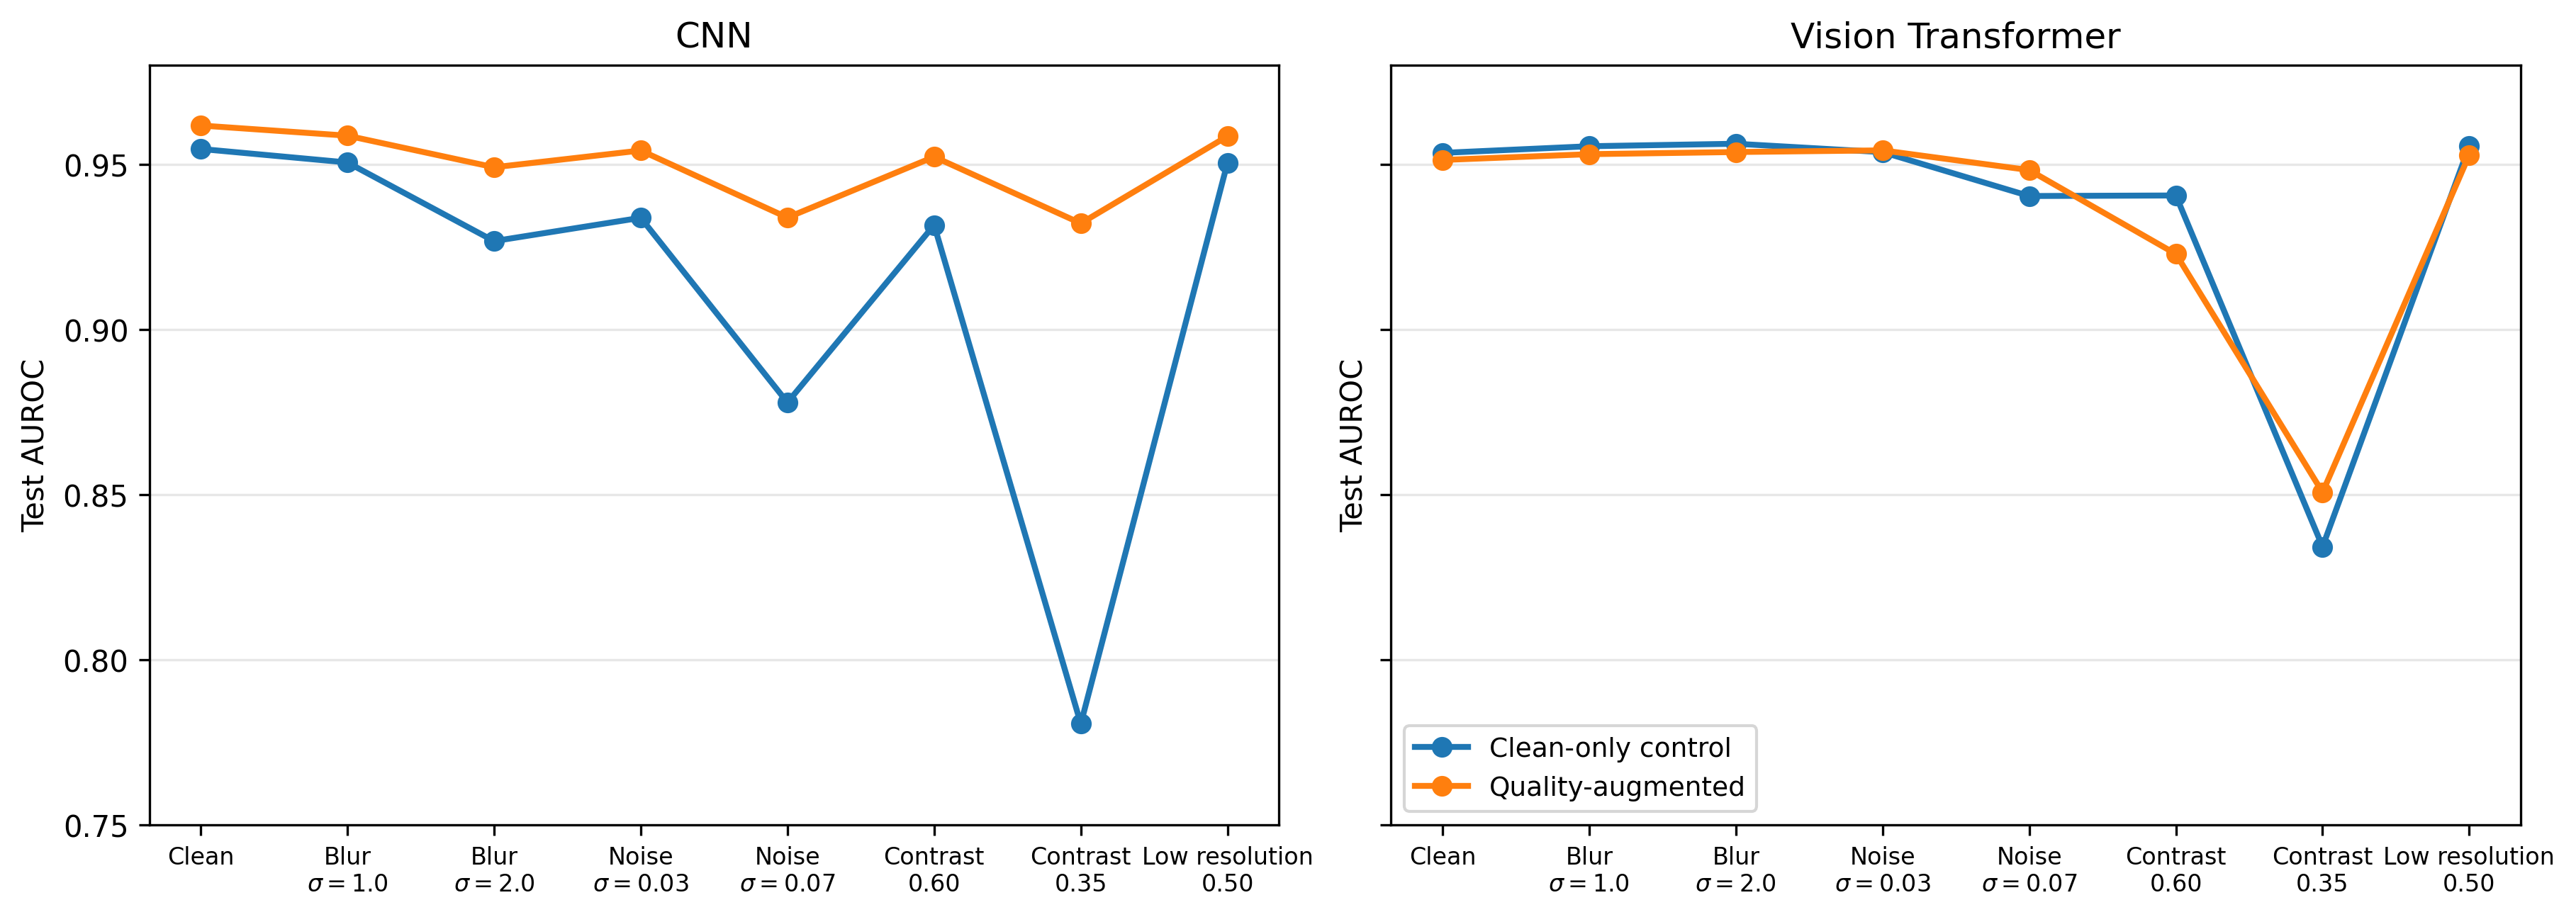
\includegraphics[width=0.96\textwidth]{figures/robustness_auroc_comparison.png}
\caption{AUROC across clean and degraded test conditions. Quality-aware augmentation raises CNN AUROC in every degraded condition, especially under severe contrast loss. It does not improve the ViT's mean degraded AUROC, although it modestly improves its performance under severe noise and severe contrast loss.}
\label{fig:results}
\end{figure*}

\subsection{Result interpretation}

Within the CNN, quality-aware augmentation increased mean degraded AUROC by 0.041 (0.907 to 0.948) and improved AUROC in every degraded condition. The largest improvement occurred under severe contrast reduction, where AUROC rose from 0.781 to 0.932; substantial gains also occurred under severe noise (0.878 to 0.934). CNN clean AUROC increased by 0.007, so H1 and H2 are both supported for the CNN under this protocol. For the ViT, the mean degraded AUROC was essentially unchanged (0.934 to 0.934; unrounded change $-0.0001$), so H1 is not supported. Its clean AUROC decreased by 0.002, within the pre-specified 0.02 margin, supporting H2. Severe contrast reduction caused the largest absolute performance drop for both architectures, even after augmentation. The comparison is based on one seed and synthetic corruptions; it should be interpreted as evidence about this benchmark protocol, not as a clinical robustness guarantee.

\section{Limitations and responsible interpretation}

This study has several limitations. PneumoniaMNIST is relatively small and derives from a pediatric chest-X-ray source, so the results may not transfer to adult populations, other hospitals, or other imaging protocols. The quality degradations are synthetic approximations rather than naturally acquired low-quality radiographs. Quality statistics can be entangled with disease appearance, and the label distribution is imbalanced. The study uses a fixed train/validation/test split, a single pre-specified seed, and no external-hospital validation; consequently, it does not estimate variability across seeds or institutions. Furthermore, 0.5 was used as a fixed threshold for the thresholded metrics without clinical threshold calibration. The models should therefore not be interpreted as clinically deployable diagnostic systems.

\section{Conclusion}

This project evaluates whether quality-aware data augmentation improves robustness of pneumonia classification to controlled chest-X-ray degradation while retaining clean-image performance. By comparing clean-only and augmented CNN and ViT models on identical clean and corrupted test images, the experiment separates performance on the target task from sensitivity to image-quality shift. For the compact CNN, the selected augmentation policy improved mean degraded AUROC by 0.041 while increasing clean AUROC by 0.007. For the ViT, it preserved clean AUROC within 0.002 but produced no aggregate robustness improvement. Thus, quality-aware augmentation can improve robustness, but its benefit is architecture-dependent in this benchmark. Future work should repeat the study across multiple seeds, validate on naturally degraded and external chest-radiograph data, and investigate augmentation policies tailored to the ViT.

\bibliographystyle{plainnat}
\bibliography{references}

\appendix
\section{Implementation checklist}

\begin{itemize}
    \item Record the command, package versions, hardware, and elapsed time for every final run.
    \item Retain the JSON metrics, history CSV, prediction archive, and plotted figures for reproducibility.
    \item Verify that every reported value comes from the test split only once per planned model configuration.
    \item Before submission, replace all \texttt{TBD} fields, add lecture slides and timestamps, and check every citation against the bibliography.
\end{itemize}

% The official template may supply checklist.tex. This makes it optional for a course report.
\IfFileExists{checklist.tex}{\newpage\input{checklist.tex}}{}

\end{document}
